\documentclass[a4paper,11pt]{article}
\usepackage{mathpazo}
\usepackage{tikz}
\usetikzlibrary{shapes}
\oddsidemargin -0.54cm
\textwidth 17.00cm
\textheight 24cm
\topmargin -1.3cm
\parindent 0pt
\parskip 1ex
\pagestyle{empty}
\begin{document}
\medskip\hrule\medskip

2 1 are inserted 

In sorted order: 1 2 

Average depth = 0.500, size 2

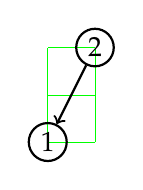
\begin{tikzpicture}[scale=0.600]
\draw [help lines, color=green] (1,-2) grid (2,0);

\draw [thick] (1,-2) node[draw, rounded rectangle] (0) {1};
\draw [thick] (2,0) node[draw, rounded rectangle] (1) {2};
\draw [->, thick] (1) to (0);

\end{tikzpicture}

\medskip\hrule\medskip
\end{document}